
\section{Experiments}

In this section, we first demonstrate the effectiveness of DU-Net through its comparison with the stacked U-Nets. Then we explore the relation between the prediction accuracy and $order$-$K$ connectivity. After that, we evaluate the iterative refinement to halve DU-Net parameters. Finally, we test the network quantization. Different combinations of bit-widths to find appropriate ones which balance accuracy, model size and memory consumption. The general comparisons are given at last. Some qualitative results are shown in Figure \ref{fig:pose-face-qualitive}.

{\bf Network.} The input resolution is normalized to 256$\times$256. Before the DU-Net, a Conv($7\times 7$) filter with stride 2 and a max pooling would produce 128 features with resolution 64$\times$64. Hence, the maximum resolution of DU-Net is 64$\times$64. Each block in DU-Net has a bottleneck structure as shown on the right side of Figure \ref{fig:framework}. At the beginning of each bottleneck, features from different connections are concatenated and stored in a shared memory. Then the concatenated features are compressed by the Conv($1\times 1$) to 128 features. At last, the Conv($3\times 3$) further produces 32 new features. The batch norm and ReLU are used before the convolutions. 

{\bf Training.} We implement the DU-Net using the PyTorch. The DU-Net is trained by the optimizer RMSprop. When training human pose estimators, the initial learning rate is $2.5\times 10^{-4}$ which is decayed to $5\times 10^{-5}$ after 100 epochs. The whole training takes 200 epochs. The facial landmark localizers are easier to train. Also starting from $2.5\times 10^{-4}$, its learning rate is divided by 5, 2 and 2 at epoch 30, 60 and 90 respectively. The above settings remain the same for quantized
DU-Net. In order to match the pace of dataflow, we set the same bit-width for gradients and inputs. We quantize dataflows and parameters all over the DU-Net except the first and last convolutional layers, since localization is a fine-grained task requires high precision of heatmaps.

{\bf Human Pose Datasets.} We use two benchmark human pose estimation datasets: MPII Human Pose \cite{andriluka14cvpr} and Leeds Sports Pose (LSP) \cite{johnson2010lsp}. The {\bf MPII} is collected from YouTube videos with a broad range of human activities. It has 25K images and 40K annotated persons, which are split into a training set of 29K and a test set of 11K. Following \cite{tompson2015efficient}, 3K samples are chosen from the training set as validation set. Each person has 16 labeled joints. The {\bf LSP} dataset contains images from many sport scenes. Its extended version has 11K training samples and 1K testing samples. Each person in LSP has 14 labeled joints. Since there are usually multiple people in one image, we crop around each person and resize it to 256x256. We also use scaling (0.75-1.25), rotation (-/+30) and random flip to augment the data.

{\bf Facial Landmark Datasets.} The experiments of the facial lanmark localization are conducted on the composite of HELEN, AFW, LFPW and IBUG which are re-annotated in the 300-W challenge \cite{sagonas2013300}. Each face has 68 landmarks. Following \cite{zhu2015face} and \cite{lv2017deep}, we use the training images of HELEN, LFPW and all images of AFW, totally 3148 images, as the training set. The testing is done on the common subset (testing images of HELEN and LFPW), challenge subset (all images from IBUG) and their union. We use the provided bounding boxes from the 300-W challenge to crop faces. The same augmentations of scaling and rotation as in human pose estimation are applied.

{\bf Metric.} We use the standard metrics in both human pose estimation and face alignment. Specifically, Percentage of Correct Keypoints (PCK) is used to evaluate approaches for human pose estimation. And the normalized mean error (NME) is employed to measure the performance of localizing facial landmarks. Following the convention of 300-W challenge, we use the inter-ocular distance to normalize mean error. For network quantization, we propose the balance index (BI) to examine the trade-off between performance and efficiency.

% \begin{table}[t!]
% \begin{center}
% \small
% % \setlength\tabcolsep{1.5pt}
% \caption{DU-Net {\it v.s.} stacked U-Nets on MPII validation set measured by PCKh and number of model parameters. With the same number of U-Nets, DU-Net achieves comparable performance as stacked U-Nets. But it has only about 30\% parameters of stacked U-Nets. The feature reuse across U-Nets make each U-Net become light-weighted.}\label{tb:hg-vs-du-nets}
% \begin{tabular}{|c|c|c|c|}
% \hline
% Method & PCKh & \# Parameters & \# Para. Ratio\\
% \hline
% \hline
% Stacked U-Nets (16) & - & 50.5M & 100\% \\
% DU-Net (16) & 89.9 & 15.9M & 31.5\% \\
% \hline
% \hline
% Stacked U-Nets (8) & 89.3 & 25.5M & 100\%\\
% DU-Net (8) & 89.5 & 7.9M & 31.0\% \\
% \hline
% \hline
% Stacked U-Nets (4) & 88.3 & 12.9M & 100\%\\
% DU-Net (4) & 88.2 & 3.9M & 30.2\% \\
% \hline
% \end{tabular}
% \end{center}
% % \vspace{-10pt}
% % \vspace{-2mm}
% \end{table}

\begin{table}[t]
\minipage[t]{0.49\textwidth}
\centering
%   \small
% \setlength\tabcolsep{1.5pt}
\caption{$Order$-1 DU-Net {\it v.s.} stacked U-Nets on MPII validation set measured by PCKh(\%) and parameter number. $Order$-1 DU-Net achieves comparable performance as stacked U-Nets. But it has only about 30\% parameters of stacked U-Nets. The feature reuse across U-Nets make each U-Net become light-weighted.}\label{tb:hg-vs-du-nets}
% \vspace*{2mm}
\begin{adjustbox}{width=1\textwidth}
\begin{tabular}{lccc}
\toprule
\multirow{2}{*}{Method} & PCKh & \#  & Parameter \\
& & Parameters & Ratio\\
\hline
% \hline
Stacked U-Nets(16) & - & 50.5M & 100\% \\
DU-Net(16) & 89.9 & 15.9M & 31.5\% \\
\hline
% \hline
Stacked U-Nets(8) & 89.3 & 25.5M & 100\%\\
DU-Net(8) & 89.5 & 7.9M & 31.0\% \\
\hline
% \hline
Stacked U-Nets(4) & 88.3 & 12.9M & 100\%\\
DU-Net(4) & 88.2 & 3.9M & 30.2\% \\
\bottomrule
\end{tabular}
\end{adjustbox}
\endminipage \hfill
\minipage[t]{0.49\textwidth}
\centering
% \small
\caption{NME(\%) on 300-W using $Order$-1 DU-Net(4) with iterative refinement, detection and regression supervisions. The top two and bottom three rows are non-iterative and iterative results. Iterative refinement could lower localization errors. Besides, the regression supervision outperforms the detection supervision.}
\label{tb:iter}
% \small
\begin{adjustbox}{width=1\textwidth}
\begin{tabular}{lcccc}
\toprule
\multirow{2}{*}{Method} & Easy  & Hard  & Full & \#\\
&Subset & Subset & Set & Para.\\
\hline
Detection only & 3.63 & 5.60 & 4.01 & 3.9M\\
Regression only &  2.91 & 5.12 & 3.34 & 3.9M\\
\hline
Detection Detection & 3.52 & 5.59 & 3.93 & 4.1M\\
Detection Regression & 2.95 & 5.12 & 3.37 & 4.1M\\
Regression Regression  & 2.87 & 4.97 & 3.28 & 4.1M\\
\bottomrule
\end{tabular} \hfill
\end{adjustbox}
\endminipage
\end{table}


% \begin{figure}[t!]
% \centering
%   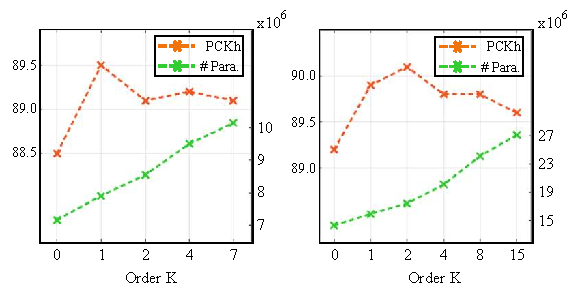
\includegraphics[width=\linewidth]{figures/exp-order-k-cropped.pdf}
% \caption{Relation of PCKh, \# parameters and $order$-$K$ connectivity on MPII validation set. The parameter number of DU-Net grows approximately linearly with the order of connectivity. However, the PCKh first increases and then decreases. A small order 1 or 2 would be a good balance for prediction accuracy and parameter efficiency.}
% \label{fig:exp-order-k}
% \end{figure}

%\subsection{Comparison with Stacked Hourglasses}
\subsection{DU-Net {\it vs.} Stacked U-Nets}
To demonstrate the advantages of DU-Net, we first compare it with traditional stacked U-Nets. This experiment is done on the MPII validation set. All DU-Nets use the $order$-$1$ connectivity and intermediate supervisions. Table \ref{tb:hg-vs-du-nets} shows three pairs of comparisons with 4, 8 and 16 U-Nets. Both their PCKh and number of convolution parameters are reported. We could observe that, with the same number of U-Nets, DU-Net could obtain comparable or even better accuracy. More importantly, the number of parameters in DU-Net is decreased by about 70\% of that in stacked U-Nets. The feature reuse across U-Nets make each U-Net in DU-Net become light-weighted. Besides, the high parameter efficiency makes it possible to train 16 $order$-$1$ connected U-Nets in a 12G GPU with batch size 16. In contrast, training 16 stacked U-Nets is infeasible. Thus, $order$-$1$ together with intermediate supervisions could make DU-Net obtain accurate prediction as well as high parameter efficiency, compared with stacked U-Nets.
% This demonstrates that the parameter efficiency is significantly improved by the order-1 connectivity.
% \begin{figure}[hbt]This is because each U-Net in DU-Net has much fewer parameters than that in stacked hourglasses.
% \centering
%   \includegraphics[width=\linewidth]{figures/unets-vs-hgs-cropped.pdf}
% \caption{}
% \label{fig:dunets-vs-hgs}
% \end{figure}

% \begin{table}[t!]
% \begin{center}
% \caption{NME(\%) on 300-W using DU-Net(4) with iterative refinement, detection and regression supervisions. The top two and bottom three rows are non-iterative and iterative results. Iterative refinement could lower facial landmark localization errors. Besides, regression supervision outperforms detection supervision.}
% \label{tb:iter}
% \small
% % \setlength\tabcolsep{1.5pt}
% \begin{tabular}{lcccc}
% \toprule
% \multirow{2}{*}{Method} & Easy  & Hard  & Full & \#\\
% &Subset & Subset & Set & Para.\\
% \hline
% Detection only & 3.63 & 5.60 & 4.01 & 3.9M\\
% Regression only &  2.91 & 5.12 & 3.34 & 3.9M\\
% \hline
% Detection Detection & 3.52 & 5.59 & 3.93 & 4.1M\\
% Detection Regression & 2.95 & 5.12 & 3.37 & 4.1M\\
% Regression Regression  & 2.87 & 4.97 & 3.28 & 4.1M\\
% \bottomrule
% \end{tabular}
% \end{center}
% \vspace{-10pt}
% % \vspace{-2mm}
% \end{table}

%\subsection{Comparison of Variable Order connectivity}
\subsection{Evaluation of $Order$-$K$ connectivity}
The proposed $order$-$K$ connectivity is key to improve the parameter efficiency of DU-Net. In this experiment, we investigate how the PCKh and convolution parameter number change along with the order value. Figure \ref{fig:exp-order-k} gives the results from MPII validation set. The left and right figures show results of DU-Net with 8 and 16 U-Nets. It is clear that the convolution parameter number increases as the order becomes larger. However, the left and right PCKh curves have a similar shape of first increasing and then decreasing. $Order$-$1$ connectivity is always better than $order$-$0$. 

However, very dense connections may not be a good choice, which is kind of counter-intuitive. This is because the intermediate supervisions already provide additional gradients. Too dense connections make gradients accumulate too much, causing the overfitting of training set. Further evidence of overfitting is shown in Table \ref{tb:overfitting}. The $order$-7 connectivity has the higher training PCKh the $order$-1 in all training epochs. But its validation PCKh is a little lower in the last training epochs. Thus, small orders are recommended in DU-Net.

% \begin{table}[htb]
% \begin{center}
% \small
% \setlength\tabcolsep{1.5pt}
% \begin{tabular}{@{}lcccccccc@{}}
% % \begin{tabular}{@{}p{2.5cm} p{0.4cm} p{0.4cm}  p{0.4cm}  p{0.4cm} p{0.4cm} p{0.4cm} p{0.4cm} p{0.4cm}@{}}
% \toprule
% Order & Head & Sho. & Elb. & Wri. & Hip & Knee & Ank. & Mean\\
% \hline
% K=0 & 96.5 & 95.4 & 89.3 & 84.4 & 88.7 & 84.7 & 80.8 & 88.5\\
% K=1 & 96.9 & 95.9 & 90.3 & 85.7 & 89.3 & 86.0 & 82.2 & 89.5\\
% K=2 & 96.8 & 95.6 & 90.6 & 85.3 & 88.9 & 84.6 & 81.6 & 89.1\\
% K=4 & 96.7 & 95.6 & 90.1 & 85.6 & 89.1 & 85.4 & 82.2 & 89.2\\
% K=7 & 96.7 & 96.0 & 90.0 & 85.3 & 88.4 & 85.0 & 82.1 & 89.1\\
% \bottomrule
% \end{tabular}
% \end{center}
% \vspace{-10pt}
% \caption{}
% \label{tb:max7}
% % \vspace{-2mm}
% \end{table}

% \begin{table}[htb]
% \begin{center}
% \small
% \setlength\tabcolsep{1.5pt}
% \begin{tabular}{@{}lcccccccc@{}}
% % \begin{tabular}{@{}p{2.5cm} p{0.4cm} p{0.4cm}  p{0.4cm}  p{0.4cm} p{0.4cm} p{0.4cm} p{0.4cm} p{0.4cm}@{}}
% \toprule
% Order & Head & Sho. & Elb. & Wri. & Hip & Knee & Ank. & Mean\\
% \hline
% K=0 & 96.5 & 95.9 & 90.0 & 85.1 & 89.5 & 85.3 & 82.0 & 89.2\\
% K=1 & 96.8 & 96.1 & 90.7 & 86.1 & 89.6 & 87.0 & 82.9 & 89.9\\
% K=2 & 96.8 & 96.0 & 91.0 & 86.8 & 89.4 & 87.1 & 83.3 & 90.1\\
% K=4 & 96.7 & 96.1 & 90.9 & 86.7 & 89.5 & 86.2 & 82.7 & 89.8\\
% K=8 & 96.7 & 96.0 & 90.9 & 86.6 & 89.3 & 86.7 & 82.4 & 89.8\\
% K=15 & 96.4 & 96.1 & 90.6 & 86.3 & 89.0 & 86.1 & 83.0 & 89.6\\
% \bottomrule
% \end{tabular}
% \end{center}
% \vspace{-10pt}
% \caption{}
% \label{tb:max15}
% % \vspace{-2mm}
% \end{table}

\begin{figure}[t]
\minipage[t]{0.49\textwidth}
\centering
  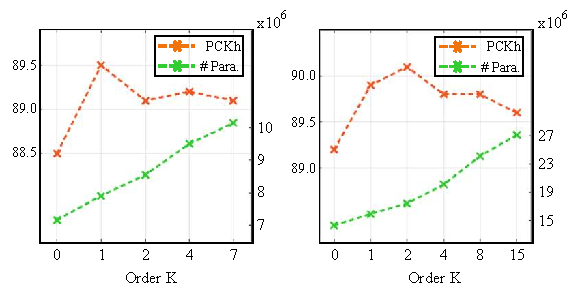
\includegraphics[width=1\linewidth]{figures/exp-order-k-cropped.pdf}
%   \vspace*{-1mm}
  \caption{Relation of PCKh(\%), \# parameters and $order$-$K$ connectivity on MPII validation set. The parameter number of DU-Net grows approximately linearly with the order of connectivity. However, the PCKh first increases and then decreases. A small order 1 or 2 would be a good balance for prediction accuracy and parameter efficiency.}
\label{fig:exp-order-k}
\endminipage \hfill
\minipage[t]{0.49\textwidth}
\centering
  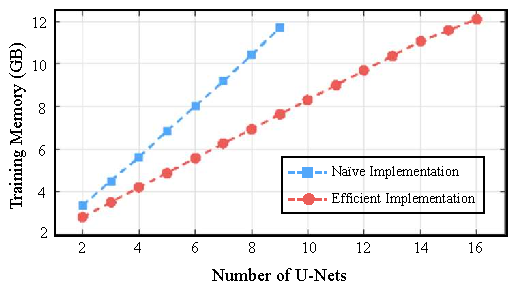
\includegraphics[width=0.9\linewidth]{figures/exp-naive-vs-efficient-cropped.pdf}
%   \vspace*{1mm}
  \caption{Naive implementation {\it v.s.} memory-efficient implementation. The $order$-$1$ connectivity, batch size 16 and a 12GB GPU are used. The naive implementation can only support 9 U-Nets at most. In contrast, the memory-efficient implementation allows to train 16 U-Nets, which nearly doubles the depth of DU-Net.}
  \label{fig:exp-naive-vs-efficient} \hfill
\endminipage
\end{figure}

% \begin{figure}[t!]
% \centering
%   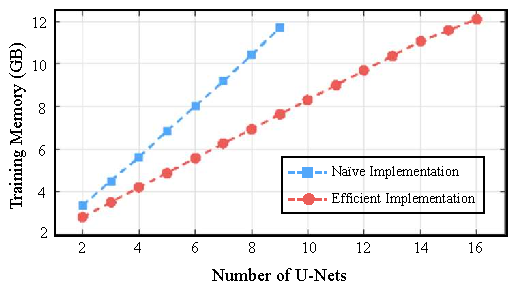
\includegraphics[width=.9\linewidth]{figures/exp-naive-vs-efficient-cropped.pdf}
% \caption{Naive implementation {\it v.s.} memory-efficient implementation. The $order$-$1$ connectivity, batch size 16 and a 12GB GPU are used. The naive implementation can only support 9 U-Nets at most. In contrast, the memory-efficient implementation allows to train 16 U-Nets, which nearly doubles the depth of DU-Net.}
% % Because of the fixed order connectivity, the training memory of naive implementation also grows linearly, but with an obviously larger slope, compared with that of memory-efficient implementation.
% \label{fig:exp-naive-vs-efficient}
% \end{figure}

\begin{table}[t]
\minipage[t]{0.49\textwidth}
\centering
%   \small
\setlength\tabcolsep{4pt}
\caption{$Order$-1 DU-Net(8) {\it v.s.} $order$-7 DU-Net(8), measured by training and validation PCKhs(\%) on MPII. $Order$-7 DU-Net(8) overfits the training set a little bit. Its validation PCKh is lower at last, though it always has higher training PCKh.}\label{tb:overfitting}
% \vspace*{2mm}
\begin{adjustbox}{width=1\textwidth}
\begin{tabular}{l|cccc}
\toprule
\multicolumn{5}{c}{PCKh on training set}\\
\hline
Epoch & 1 & 50 & 100 & 150 \\
\hline
$Order$-1 DU-Net(8) & 20.3 & 83.2 & 87.7 & 91.7 \\
$Order$-7 DU-Net(8) & {\bf 25.2} & {\bf 84.7} & {\bf 89.3} & {\bf 93.1} \\
\hline
\multicolumn{5}{c}{PCKh on validation set}\\
\hline
Epoch & 1 & 50 & 100 & 150 \\
\hline
$Order$-1 DU-Net(8) & 29.4 & 82.8 & {\bf 85.7} & {\bf 87.1}\\
$Order$-7 DU-Net(8) & {\bf 36.6} & {\bf 84.0} & 85.1 & 86.7\\
\bottomrule
\end{tabular}
\end{adjustbox}
\endminipage \hfill
\minipage[t]{0.49\textwidth}
\centering
% \small
\caption{Iterative $order$-1 DU-Net(4) {\it v.s.} non-iterative $order$-1 DU-Net(8) on 300-W measured by NME(\%). Iterative DU-Net(4), with few additional parameters on DU-Net(4), achieves comparable performance as DU-Net(8). Thus, the iterative refinement has the potential to halve parameters of DU-Net but still maintain comparable performance.}
% \small
\begin{adjustbox}{width=1\textwidth}
\label{tb:iter4-vs-8}
\begin{tabular}{lcccc}
\toprule
\multirow{2}{*}{Method} & Easy  & Hard  & Full & \#\\
&Subset & Subset & Set & Parameters\\
\hline
DU-Net(4) &  2.91 & 5.12 & 3.34 & 3.9M\\
Iter. DU-Net(4)  & 2.87 & 4.97 & 3.28 & 4.1M\\
DU-Net(8) & 2.82 & 5.07 & 3.26 & 7.9M\\
\bottomrule
\end{tabular} \hfill
\end{adjustbox}
\endminipage
\end{table}

\subsection{Evaluation of Efficient Implementation}

The memory-efficient implementation makes it possible to train very deep DU-Net. Figure \ref{fig:exp-naive-vs-efficient} shows the training memory consumption of both naive and memory-efficient implementations of DU-Net with order-1 connectivity. The linear growths of training memory along with number of U-Nets is because of the fixed order connectivity. But the memory growth of efficient implementation is much slower than that of the naive one. With batch size 16, we could train a DU-Net with 16 U-Nets in 12GB GPU. Under the same setting, the naive implementation could accept only 9 U-Nets.


%\subsection{Exploration of Iterative Estimation}
\subsection{Evaluation of Iterative Refinement}
% The iterative refinement is proposed to improve the landmark localization accuracy with few additional parameters.
The iterative refinement is designed to make DU-Net more parameter efficient. First, experiments are done on the 300-W dataset using DU-Net(4). Results are shown in Table \ref{tb:iter}. For both detection and regression supervisions, adding an iteration could lower the localization errors, demonstrating effectiveness of the iterative refinement. Meanwhile, the model parameters only increase 0.2M, making DU-Net even more parameter efficient. Besides, the regression supervision outperforms the detection one no matter in the iterative or non-iterative setting, making it a better choice for landmark localization. 
% Thus, regression supervision is more suitable for landmark localization tasks. 

Further, we compare iterative DU-Net(4) with non-iterative DU-Net(8). Table \ref{tb:iter4-vs-8} gives the comparison. We could find that, the iterative DU-Net(4) could obtain comparable NME as DU-Net(8). However, DU-Net(8) has double parameters of  DU-Net(4) whereas iterative DU-Net(4) increases only 0.2M additional parameters on DU-Net(4).


\subsection{Evaluation of Network Quantization}

Through network quantization, high precision operations and parameters can be efficiently represented by a few discrete values. 
In order to find appropriate choices of bit-widths, we try a series of bit-width combinations on the 300-W dataset based on $order$-$1$ DU-Net(4). The performance and balance ability of these combinations on several methods are shown in Table \ref{tb:IWG-QUAN}, where DU-Net(4) is DU-Net with 4 blocks, BW and TW respectively represents binarized weight and ternarized weight without $\alpha$, BW-$\alpha$ is binarized weight with float scaling factor $\alpha$, the suffix QIG means quantized inputs and gradients. 

For mobile devices with limited computational resources, slightly performance drop is tolerable provided that corresponding large efficiency enhancement. For the evaluation purpose, we propose a balance index (BI) to better examine the trade-off between performance and efficiency: 
\begin{equation} \label{eq:bi}
BI = NME^2 \cdot TM \cdot MS  
\end{equation} 
where $TM$ and $MS$ is respectively short for training memory and model size compression ratios to the original network without quantization. The square of $NME$ is calculated in the above formula to emphasize the prior importance of performance. For BI, the smaller the value, the better the ability of balance.

According to Table \ref{tb:IWG-QUAN}, BW-QIG(818) could achieve the best balance between performance and model efficiency among all the combinations. BW-QIG(818) could reduce more than 4$\times$ training memory and 32$\times$ model size while reach a better performance than TSR \cite{lv2017deep}. Besides, BW-$\alpha$-QIG(818),  BW-QIG(616) and TW-QIG(626) also have small balance index. Among all the combinations, the binarized network with scaling factor $\alpha$, i.e. BW-$\alpha$ gets the closest error to the original network DU-Net(4).


For BW-$\alpha$-QIG(818), the performance is not better than BW-QIG(818). This is mainly because that BW-$\alpha$ is heavily rely on the parameter $\alpha$. However, the quantization of dataflow could reduce the approximation ability of $\alpha$. TW and TW-QIG usually gets better results than BW and BW-QIG, since they have more choices in terms of weight value. The above results proves the effectiveness of network quantization, yet a correct combination of bit-widths is a crucial factor.


\begin{table}[t!]
\begin{center}
\caption{Performance and balance ability of different combinations of bit-width values on the 300-W dataset measured by NME(\%), all quantized networks are based on $order$-$1$ DU-Net(4). BW and TW is short for binarized and ternarized weight, $\alpha$ represents float scaling factor, QIG is short for quantized inputs and gradients. $Bit_I$, $Bit_W$, $Bit_G$ represents the bit-width of inputs, weights, gradients respectively. Training memory and model size is represented by the compression ratio to the original DU-Net(4). Balance index is calculated by equation \ref{eq:bi}. Comparable error rate could be achieved by binarized the model parameters. Further quantizing the inputs and gradients could substantially reduce the training memory with some increase of detection error. The balance index is a indicator for balancing the quantization and accuracy.}
%The binarized network with scaling factor $\alpha$ gets the closest error to the original network. Taking the quantization of inputs and gradients into consideration, binarized network trained with 8-bits quantized inputs and gradients has the lowest balance index.

\small
% \setlength\tabcolsep{1.5pt}
% \label{tb:IWG-QUAN}
% \begin{tabular}{lccccccc}
% \toprule
% % Method & $Bit_I$  & $Bit_W$  & $Bit_G$ & NME(\%)  \\
% \multirow{2}{*}{Method} & {$Bit_I$}  & $Bit_W$  & $Bit_G$ & NME & Training  &  Model & Balance\\
% & & & & (\%) & Memory & Size & Index\\

% % & Training Memory & 
% \hline
% DU-Net(4)  &  32  & 32  & 32  & 3.38 & 1.00 & 1.00 & 11.4 \\
% \hline
% BW-QIG     &  6   & 1   & 6   & 5.93 & 0.17 & 0.03 & 0.18	\\
% BW-QIG     &  8   & 1   & 8   & 4.30 & 0.25 & 0.03 & \bf{0.14}	    \\
% BW-$\alpha$-QIG    &  8   & 1   & 8   & 4.47 & 0.25 & 0.03 & 0.15  \\
% BW         &  32  & 1   & 32  & 3.75 & 1.00 & 0.03 & 0.42	\\
% BW-$\alpha$        &  32  & 1   & 32  & {\bf 3.58} & 1.00 & 0.03 & 0.38  \\
% TW         &  32  & 2   & 32  & 3.73 & 1.00 & 0.06 & 0.83  \\
% TW-QIG     &  6   & 2   & 6   & 4.27 & 0.17 & 0.06 & 0.19	\\
% TW-QIG     &  8   & 2   & 8   & 4.13 & 0.25 & 0.06 & 0.26   \\


% \bottomrule
% \end{tabular}

\label{tb:IWG-QUAN}
\begin{tabular}{lccccccccc}
\toprule
% Method & $Bit_I$  & $Bit_W$  & $Bit_G$ & NME(\%)  \\
\multirow{2}{*}{Method} & {$Bit_I$}  & $Bit_W$  & $Bit_G$ & NME(\%) & NME(\%) & NME(\%) & Training  &  Model & Balance\\
& & & & Full set & Easy set & Hard set & Memory & Size & Index\\

% & Training Memory & 
\hline
DU-Net(4)  &  32  & 32  & 32  & 3.38 & 2.95 & 5.13 & 1.00 & 1.00 & 11.4 \\
\hline
BW-QIG     &  6   & 1   & 6   & 5.93 & 5.10 & 9.34 & 0.17 & 0.03 & 0.18	\\
BW-QIG     &  8   & 1   & 8   & 4.30 & 3.67 & 6.86 & 0.25 & 0.03 & \bf{0.14}	    \\
BW-$\alpha$-QIG    &  8   & 1   & 8   & 4.47 & 3.75 & 7.40 & 0.25 & 0.03 & 0.15  \\
BW         &  32  & 1   & 32  & 3.75 & 3.20 & 5.99 & 1.00 & 0.03 & 0.42	\\
BW-$\alpha$        &  32  & 1   & 32  & {\bf 3.58} & 3.12 & 5.45 & 1.00 & 0.03 & 0.38  \\
TW         &  32  & 2   & 32  & 3.73 & 3.21 & 5.85 & 1.00 & 0.06 & 0.83  \\
TW-QIG     &  6   & 2   & 6   & 4.27 & 3.70 & 6.59 & 0.17 & 0.06 & 0.19	\\
TW-QIG     &  8   & 2   & 8   & 4.13 & 3.55 & 6.50 & 0.25 & 0.06 & 0.26   \\
\bottomrule
\end{tabular}

\end{center}
% \vspace{-10pt}
% \vspace{-2mm}
\end{table}

\begin{table}[htb]
\begin{center}
\small
\caption{Comparison of convolution parameter number (Million) and model size (Megabyte) with state-of-the-art methods. DU-Net(16) has 27\%-62\% parameters of other methods. Its binarized version DU-Net-BW-$\alpha$(16) has less than {\bf 2\%} model size.}\label{tb:para-num}
\setlength\tabcolsep{0.5pt}
\begin{tabular}{lccccc|cc}
\toprule
\multirow{2}{*}{Method} & Yang  & Wei & Bulat  & Chu & Newell  & $Order$-1 & $Order$-1 DU-\\
& {\it et al.}\cite{yang2017learning} & {\it et al.}\cite{wei2016convolutional}  
& {\it et al.}\cite{bulat2016human} & {\it et al.}\cite{chu2017multi} & {\it et al.}\cite{newell2016stacked} & DU-Net(16) & Net-BW-$\alpha$(16)\\
\hline
\# Parameters & 28.0M & 29.7M & 58.1M & 58.1M & 25.5M & {\bf 15.9M} & {\bf 15.9M}\\
Model Size & 110.2MB & 116.9MB & 228.7MB & 228.7MB & 100.5MB & 62.6MB & {\bf 2.0MB}\\

% \hline
% \cite{yang2017learning} & \\
% \cite{wei2016convolutional} & \\
% \cite{bulat2016human} & \\
% \cite{chu2017multi} & \\
% % Carreira \textit{et al.}\cite{carreira2016human} & 10.0M\\
% % \cite{belagiannis2017recurrent} & 15.4M\\
% \hline
% Stacked HGs(8) \cite{newell2016stacked} & \\
% DU-Net(8) & \\
% DU-Net(16) & \\
\bottomrule
\end{tabular}
\end{center}
% \vspace{-10pt}
% \vspace{-2mm}
\end{table}

\subsection{Comparison with State-of-the-art Methods}

% We compare the DU-Net with state-of-the-art approaches for both human pose estimation and facial landmark localization.

{\bf Human Pose Estimation.}
Tables \ref{tb:mpii} and \ref{tb:lsp} show comparisons of human pose estimation on MPII and LSP test sets. The $order$-$1$  DU-Net-BW-$\alpha$(16) achieves comparable state-of-the-art performances. In contrast, as shown in Table \ref{tb:para-num}, it has only 27\%-62\% parameters and less than 2\% model size of other recent state-of-the-art methods. The DU-Net is concise and simple. Other state-of-the-art methods use stacked U-Nets with either sophisticated modules \cite{yang2017learning}, graphical models \cite{chu2017multi} or adversarial networks \cite{yu2017adversarial}.

{\bf Facial Landmark Localization.}
The DU-Net is also compared with other state-of-the-art facial landmark localization methods on 300-W. Please refer to Table \ref{tb:300w}. We uses a smaller network $order$-1 DU-Net(8) than that in human pose estimation, since localizing the facial landmarks is easier. The $order$-1 DU-Net-BW-$\alpha$(8) gets comparable errors state-of-the-art method \cite{newell2016stacked}. However, $order$-1 DU-Net-BW-$\alpha$(8) has only $\sim$2\% model size.

\begin{figure*}[t!]
\centering
  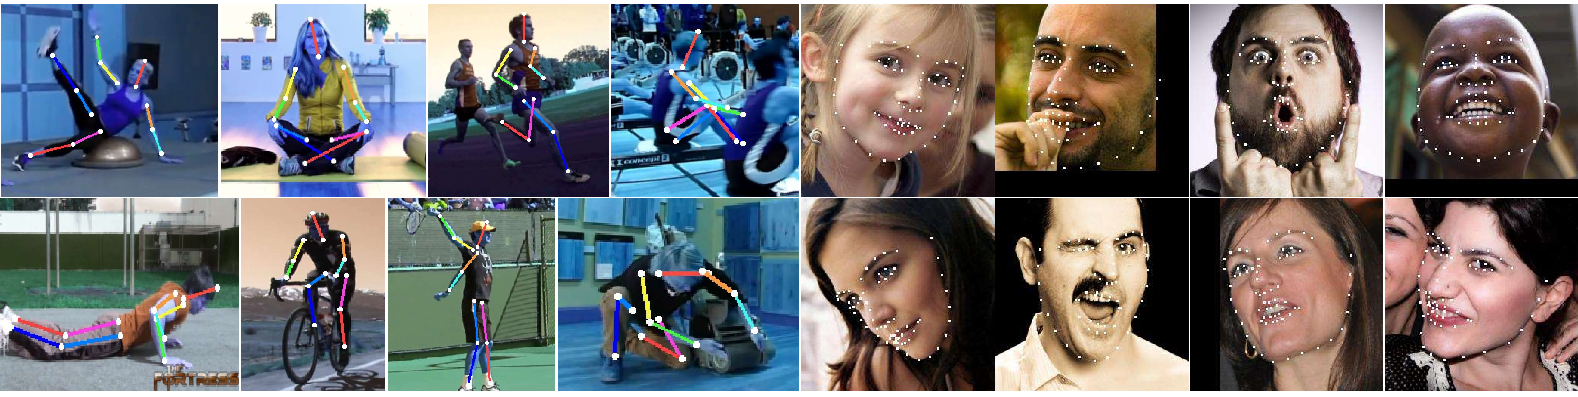
\includegraphics[width=0.9\linewidth]{figures/pose-face-qualitive-results-cropped.pdf}
\caption{Qualitative results of human pose estimation and facial landmark localization. DU-Net could handle a wide range of human poses, even with occlusions. It could also detect accurate facial landmarks with various head poses and expressions.}
\label{fig:pose-face-qualitive}
\end{figure*}

\begin{table}[t!]
\begin{center}
\small
\setlength\tabcolsep{1.5pt}
\caption{PCKh(\%) comparison on MPII test sets. $Order$-$1$ DU-Net could achieve comparable performance as state-of-the-art methods. More importantly, DU-Net-BW-$\alpha$(16) has at least $\sim${\bf 30\%} parameters and at most $\sim${\bf 2\%} model size.}\label{tb:mpii}
\begin{tabular}{@{}lcccccccc@{}}
\toprule
Method & Head & Sho. & Elb. & Wri. & Hip & Knee & Ank. & Mean\\
\hline
Pishchulin \textit{et al.} ICCV'13 \cite{pishchulin2013strong} & 74.3 & 49.0 & 40.8 & 34.1 & 36.5 & 34.4 & 35.2 & 44.1\\
Tompson \textit{et al. } NIPS'14 \cite{tompson2014joint} & 95.8 & 90.3 & 80.5 & 74.3 & 77.6 & 69.7 & 62.8 & 79.6\\
Carreira \textit{et al.} CVPR'16 \cite{carreira2016human} & 95.7 & 91.7 & 81.7 & 72.4 & 82.8 & 73.2 & 66.4 & 81.3\\
Tompson \textit{et al.} CVPR'15 \cite{tompson2015efficient}& 96.1 & 91.9 & 83.9 & 77.8 & 80.9 & 72.3 & 64.8 & 82.0\\
Hu \textit{et al.} CVPR'16 \cite{hu2016bottom}& 95.0 & 91.6 & 83.0 & 76.6 & 81.9 & 74.5 & 69.5 & 82.4\\
Pishchulin \textit{et al.} CVPR'16 \cite{pishchulin2016deepcut}&94.1 & 90.2 & 83.4 & 77.3 & 82.6 & 75.7 & 68.6 & 82.4\\
Lifshitz \textit{et al.} ECCV'16 \cite{lifshitz2016human} & 97.8 & 93.3 & 85.7 & 80.4 & 85.3 & 76.6 & 70.2 & 85.0\\
Gkioxary \textit{et al.} ECCV'16 \cite{gkioxari2016chained} & 96.2 & 93.1 & 86.7 & 82.1 & 85.2 & 81.4 & 74.1 & 86.1\\
Rafi \textit{et al.} BMVC'16 \cite{rafi2016efficient} & 97.2 & 93.9 & 86.4 & 81.3 & 86.8 & 80.6 & 73.4 & 86.3\\
Belagiannis \textit{et al.} FG'17 \cite{belagiannis2017recurrent}&97.7 & 95.0 & 88.2 & 83.0 & 87.9 & 82.6 & 78.4 & 88.1\\
Insafutdinov \textit{et al.} ECCV'16 \cite{insafutdinov2016deepercut}&96.8 & 95.2 & 89.3 & 84.4 & 88.4 & 83.4 & 78.0 & 88.5\\
Wei \textit{et al.} CVPR'16 \cite{wei2016convolutional} & 97.8 & 95.0 & 88.7 & 84.0 & 88.4 & 82.8 & 79.4 & 88.5\\
Bulat \textit{et al.} ECCV'16 \cite{bulat2016human} & 97.9 & 95.1 & 89.9 & 85.3 & 89.4 & 85.7 & 81.7 & 89.7\\
Newell {\it et al.}  ECCV'16 \cite{newell2016stacked} & 98.2 & 96.3 & 91.2 & 87.1 & 90.1 & 87.4 & 83.6 & 90.9\\
Chu \textit{et al.} CVPR'17 \cite{chu2017multi} & {\bf 98.5} & 96.3 & 91.9 & {\bf 88.1} & {\bf 90.6} & {\bf 88.0} & {\bf 85.0} & {\bf 91.5}\\
\hline
$Order$-$1$ DU-Net(16) & 97.4  & {\bf 96.4}  & {\bf 92.1}  & 87.7  & 90.2  & 87.7 & 84.3 & 91.2\\
$Order$-$1$ DU-Net-BW-$\alpha$(16) & 97.6  & 96.4  & 91.7  & 87.3  & 90.4  & 87.3 & 83.8 & 91.0\\
\bottomrule
\end{tabular}
\end{center}
% \vspace{-10pt}
% \vspace{-2mm}
\end{table}

\begin{table}[t]
\begin{center}
\caption{NME(\%) comparison with state-of-the-art facial landmark localization methods on 300-W dataset. DU-Net-BW-$\alpha$ refers to the DU-Net with binarized weights and scaling factor $\alpha$ The binarized DU-Net obtains comparable performance with state-of-the-art method \cite{newell2016stacked}. But it has $\sim${\bf 50}$\times$ smaller model size.}\label{tb:300w}
\small
\setlength\tabcolsep{0.5pt}
\begin{tabular}{lccccccc|ccc}
\toprule
\multirow{2}{*}{Method} & CFAN  & Deep  & CFSS  
& TCDCN  & MDM  & TSR & HGs(4) & $Order$-1 & $Order$-1 DU-\\
& \cite{zhang2014coarse} & Reg \cite{shi2014deep} & \cite{zhu2015face} & \cite{zhang2014facial} &  \cite{trigeorgis2016mnemonic} & \cite{lv2017deep} & \cite{newell2016stacked} & DU-Net(8)& Net(8)-BW-$\alpha$\\
\hline
Easy subset  & 5.50 & 4.51  &  4.73 & 4.80 & 4.83  & 4.36 & 2.90 & {\bf 2.82} & 3.00\\ 
Hard subset  & 16.78 &  13.80  & 9.98 & 8.60 & 10.14 &  7.56 & 5.15 &{\bf 5.07} & 5.36\\
Full set   & 7.69 & 6.31 & 5.76 & 5.54 & 5.88 & 4.99 & 3.35 & {\bf 3.26} & 3.46\\
% \hline
% Stacked HGs(4) \cite{} & 2.85 & 4.88 & 3.24\\
% Stacked HGs(4) \cite{newell2016stacked} &   &  & \\
% +$CoCoNet$ & {\bf 2.90} & {\bf 5.15} & {\bf 3.37}\\
\bottomrule
\end{tabular}
\end{center}
% \vspace{-10pt}
% \vspace{-2mm}
\end{table}

\begin{table}[htb]
\begin{center}
\small
\caption{PCK(\%) comparison on LSP test set. The $Order$-$1$ DU-Net could also obtain comparable state-of-the-art performance. But DU-Net-BW-$\alpha$(16) has at most $\sim${\bf 70}\% fewer parameters and $\sim${\bf 50}$\times$ smaller model size than other state-of-the-art methods.}\label{tb:lsp}
\setlength\tabcolsep{1.5pt}
\begin{tabular}{@{}lcccccccc@{}}
\toprule
Method & Head & Sho. & Elb. & Wri. & Hip & Knee & Ank. & Mean\\
\hline
Belagiannis \textit{et al.} FG'17 \cite{belagiannis2017recurrent} & 95.2 & 89.0 & 81.5 & 77.0 & 83.7 & 87.0 & 82.8 & 85.2\\
Lifshitz \textit{et al.} ECCV'16 \cite{lifshitz2016human} & 96.8 & 89.0 & 82.7 & 79.1 & 90.9 & 86.0 & 82.5 & 86.7\\
Pishchulin \textit{et al.} CVPR'16 \cite{pishchulin2016deepcut} &  97.0 & 91.0 & 83.8 & 78.1 & 91.0 & 86.7 & 82.0 & 87.1\\
Insafutdinov \textit{et al.} ECCV'16 \cite{insafutdinov2016deepercut}& 97.4 & 92.7 & 87.5 & 84.4 & 91.5 & 89.9 & 87.2 & 90.1\\
Wei \textit{et al.} CVPR'16 \cite{wei2016convolutional}& 97.8 & 92.5 & 87.0 & 83.9 & 91.5 & 90.8 & 89.9 & 90.5\\
Bulat \textit{et al.} ECCV'16 \cite{bulat2016human}& 97.2 & 92.1 & 88.1 & 85.2 & 92.2 & 91.4 & 88.7 & 90.7\\
Chu \textit{et al.} CVPR'17 \cite{chu2017multi}& 98.1 & 93.7 & 89.3 & 86.9 &  93.4 & 94.0 & 92.5 & 92.6\\
% Chou \textit{et al.}\cite{chou2017self} & 98.2 & 94.9 & 92.2 & 89.5 & 94.2 & 95.0 & 94.1 & 94.0\\
Newell {\it et al.} ECCV'16 \cite{newell2016stacked} & {\bf 98.2} & 94.0 & 91.2 & 87.2 & 93.5 & {\bf 94.5} & 92.6 & 93.0\\
Yang \textit{et al.} ICCV'17 \cite{yang2017learning} & {\bf 98.3} & 94.5 & 92.2 & 88.9 & {\bf 94.4} & 95.0 & 93.7 & 93.9\\
% Chou \textit{et al.}\cite{chou2017self} & 98.2 & 94.9 & 92.2 & 89.5 & 94.2 & 95.0 & 94.1 & 94.0\\
\hline
% $Order$-$1$ DU-Net(8) & 97.1 &  94.7 &  91.6 & 89.0  & 93.7  & 94.2 &  93.7  & 93.4\\
$Order$-$1$ DU-Net(16) &  97.5 & {\bf 95.0} & {\bf 92.5} & {\bf 90.1} &  93.7 &  {\bf 95.2} & 94.2 & {\bf 94.0}\\
$Order$-$1$ DU-Net-BW-$\alpha$(16) &  97.8 & 94.3 & 91.8 & 89.3 &  93.1 &  94.9 & {\bf 94.4} & 93.6\\

\bottomrule
\end{tabular}
\end{center}
% \vspace{-10pt}
% \vspace{-2mm}
\end{table}



